
%%%%%%%%%%% Nomenclature for this chapter%%%%%%%%%%
\nomenclature{UOP}{University of Paris 11}
\chapter{Internal Fine Tuning and Canonical Large Numbers}
\label{chap:chapter_1}

%%%%%%%%%%%%%%%%%%%%%%%%%%%%%%%%%%%%
%%%%%%%%%%%%%%%%%%%%%%%%%%%%%%%%%%%%

\section{The Famous Double Cosmic Fine-Tuning and the Topological Axis}
\label{sec:examples}

The most famous fine tuning implies cosmic quantities, but this is awkwardly called the `Double
Large Number Problem`. If it is a `problem` for standard evolutionary cosmology, it is a precious
clue in steady-state cosmology based on the Perfect Cosmological Principle (spatial and temporal
homogeneity) [3].
This Cosmic Fine-Tuning leads directly to a Gravitational Hydrogen model of the universe [3]
defining the Universe horizon radius $R = 2a G \lambdabar e$ , the factor 2 coming from the two atoms in
Hydrogen molecule, where $\lambdabar e = \hbar/cm e$ is the Electron Compton reduced wavelength, and the
gravitational coupling constant $a G = \hbar c/Gm H m p$ , so the speed c is eliminated. This conforms with
Coherent Cosmology which needs signal celerity far exceeding c. This gives R ≈ 13,812 Gly, corresponding to a Hubble constant 70.790 (km/s)/Megaparsec, compatible with the
most recent measurement [4]: 72(3) (km/s)/Megaparsec, which confirms the value measured
directly by the 1a type novae, while the standard optimization of 6 parameters results in a lower
value of 9 %.
Let us associate the visible universe of mass M with a matter-wave, of wavelength $\lambdabar M = \hbar /Mc = 4
10^{-96} m$. This 'Topon' is close to the touchstone n = 30 of the Topological Axis, see Fig. 1,
corresponding to $n ≈ 2e^e$ , to $0.01{percent}$ , The Topological Axis illustrates the function $f{n + 4} = f 2 {n}$
and results from the imbrication of relations of form \lambdabar e /l micro ~ (l macro /\lambdabar e ) 2 , followed by l macro /\lambdabar e ~
(\lambdabar e /l' micro ) 2 :
\lambdabar e /\lambdabar M ~ (R/ \lambdabar e ) 2 ~ ( \lambdabar e / \lambdabar X ) 4 ~ (λ CMB / \lambdabar e ) 8 ~ ( \lambdabar e / \lambdabar W ) 16 ~ (2r H / \lambdabar e ) 32 ~ ( \lambdabar e / l Gl ) 64 ~ ( \lambdabar str / \lambdabar e ) 128 ~ 2^{256}
where a string wavelength ƛ str , appears, with mass about 2 MeV. So, the correlation is octuple,
including, apart the two ones above, three relations which have been independently reported [3].
The overall large number 2^{256} has an evident computational character, confirmed below by the
dramatic appearance of the Eddington Large Number, and permits to approach each physical length.
In particular, the relation R/ \lambdabar e ~ ( CMB / \lambdabar e ) 4 ties two cosmic lengths, the Hubble radius and the CMB
wavelength by a relation incompatible with the standard vevolutionary cosmology. Of this order of
magnitude, we infer rather precise relations. First, considering the cosmological neutrino
background (CNB), whose wavelength is defined by (  CNB /  CMB ) 3 = 11/4, we have R/ \lambdabar e ~
(  CNB 2 /  CMB \lambdabar e ) 4 to $1.7{percent}$. Second, with the Hydrogen radius r H(0) = a\lambdabar e , we infer R/r H(0) ~
(4  CMB /r H(0) ) 4 precise to 0.6 %. One notes that the appearance of the neutrino field is conform
with the synthesis of the two main cosmologies, where the single Bang is replaced by a matter-
antimatter Oscillatory Bounce [5].
In particular, it was noted [1] that a G is of order W 8 , where W is the mass ratio W boson-
Electron. With the above R value, one observes the following more symmetrical relation involving
the other (neutral) weak boson Z, in the 0.01{percent} indetermination of W and Z:
$R/√(\lambdabar p \lambdabar H ) ≈ (WZ) 4$
where $\lambdabar p$ and $\lambdabar H$ are the Proton and Hydrogen reduced wavelengths. The precision of this formula
will be pulled to the ppb range in Section III, by intervention of canonical mathematical constants.
The gravitational Hydrogen molecule model [3] implies the following double correlation,
which is the simplest case of Eddington's statistical theory [2]. The position of a 'reference particle'
is supposed to be determined with an uncertainty R/2. For N particles of mass m constituting thevisible Universe, the deviance is statistically divided by √N, where N = M/m. If m is assumed to be
the effective mass of the electron in the Hydrogen atom, m' e = m e p/H, and if, moreover, we equate
the deviance R/(2√(M/m' e )) to the Hydrogen wavelength $\lambdabar H = \hbar/cm H$ , we obtain the double relation:
$R/2\lambdabar H = √(M/m' e ) = \hbar c/Gm e m p$
This is the definitive interpretation of the Double Large Number Fine-tuning. So, while the two
pillars of Physics, Relativity and Quantum Theory are unable to conciliate Gravitation and Particle
Physics, the third pillar, Statistical Physics, directly makes this connection in cosmology [2].
Recall that, contrary to what is often stated, Quantum Physics does not limit to Micro-physics.
Indeed the exclusion principle applies in both solid state physics and in stellar physics. In particular,
for a star containing N s atoms, in which the pressure has reached the quantum degeneracy value
(case of white dwarfs), exclusion principle applies for electrons, and the radius star is about R/N s1/3 .
So the formula giving the Hubble radius R, a very difficult measurement which puzzled a whole
century, was already contained in astrophysics textbooks. The universe radius amazingly appears as
the limit of a mono-atomic star radius, of which the electrons are in degeneracy state. Eddingon was
aware of this Cosmologic Exclusion Principle, but could not conclude since, at his epoch, the
Hubble measurement for R was false by an order of magnitude.
The reason for this discrepancy is that Lemaître and Hubble considered galaxies of the Local
Group, which do not participate the so-called Space expansion. In fact, it suffices to introduce a
repulsive force proportional to galaxy groups separation distance, for explaining the canonical
exponential recession. There is no need of the so-called 'dark energy', the repulsive force is simply
the cosmological constant identified to 1/R 2 . The distance for which this force exceeds attractive
gravitation between galaxies is about 10 6 light years [3], which corresponds, in the Topological
Axis, to the Atiyah Constant Γ , presented in the Section III, see Fig 1.
In the steady-state cosmology, such a repulsive force between galaxy groups is necessary, in
order to avoid a big chill due to the thermodynamics second principle. But, inside a galaxy group,
another evacuation mechanism must occur: it would be the role of massive black holes.

For instance, this paper \cite{fm1} is awesome.

See Figure \ref{fig:figure_label} as an example on how to add figures to your thesis.
It is recommended that all figures to be kept in a separate directory.
Note the `./figures/figure' in the example below.


\begin{figure}
\centering
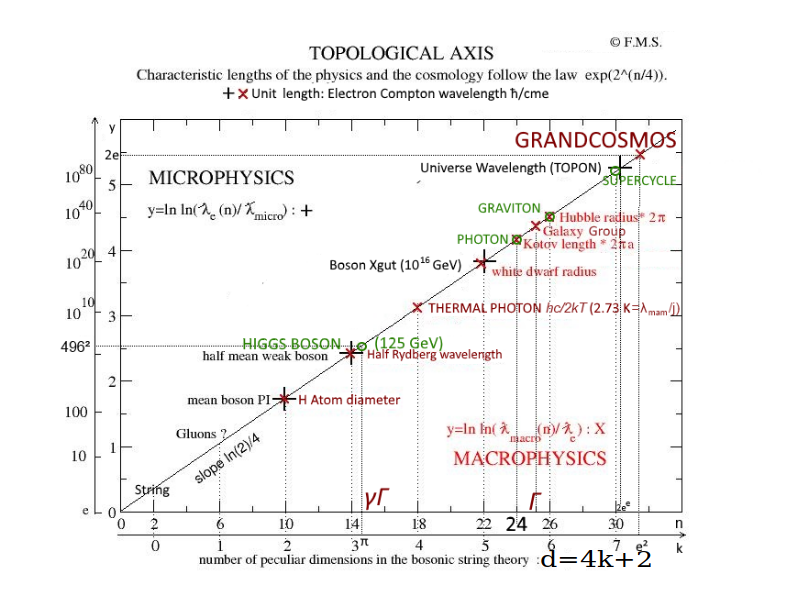
\includegraphics[width=0.5\textwidth]{./figures/figure}
\caption{A figure example.}
\label{fig:figure_label}
\end{figure}


See Table \ref{table:table_ex} to learn how to create tables.

\begin{table}
\centering
\caption{A table example}
\begin{tabular}{ c c c c }
\toprule
\textbf{Dataset} & \textbf{Number of samples} & \textbf{Results} & \textbf{Results 2} \\
\midrule                 
  Ini & 1405 & 48 & 9 \\ 
  Mid & 1196 & 52 & 10 \\ 
  Fin & 1629 & 44 & 9 \\ 
  Iso & 1372 & 39 & 8 \\ 
  \bottomrule
\end{tabular}
\label{table:table_ex} 
\end{table}

This how you create a new definition: go to \ref{def:distance_function}.

\begin{definition}
Given a data space $\mathfrak{D}$, for any two data elements $x,y \in \mathfrak{D}$, a \textbf{distance function} $dist$, on $\mathfrak{D}$ is defined as:
\begin{equation}
dist: \mathfrak{D} \times \mathfrak{D} \longrightarrow \mathds{R}_{\geq 0} 
\end{equation}
where $dist$ has the following properties:
\begin{compactitem}
\item $dist(x,y)=0 \Leftrightarrow x=y$ (reflexivity)
\item $dist(x,y) = dist(y,x)$ (symmetry)
\end{compactitem}
The pair $(\mathfrak{D},dist)$ is called a \textbf{distance space}.
\label{def:distance_function}
\end{definition}


\section {Cosmic Holography, Toponic Quantification and Cosmos vastness}

In the steady-state cosmologic model of Bondi, Gold and Hoyle, the Perfect Cosmological
Principle implies the invariance of the Universe mean mass density ρ and the exponential recession
of galaxy groups, with time constant R/c being compensated by the appearance of m n massive
neutrons at rate $c^3 /Gm n $. The invariant visible Universe radius R is then defined by the
Schwarszchild relation so that each point is the center of an equivalent R-radius black hole, of
critical mass $M = Rc 2 /2G$ and wavelength $\lambdabar M = \hbar/Mc = 2l P2 /R$, the above 'Topon'. The Bekenstein-
Hawking entropy of this black-hole Universe shows an 1D extension of the standard Holographic
Principle , only devoted to 3D application [6]:
$S BH = \pi(R/l P )2 = 2\pi R/\lambdabar M$
where $l P = (Ghbar/c^3 ) 1/2$ is the Planck's length. Note that, while the standard evolutionary cosmology
use differential equations, the steady-state Cosmology must favor such integral relations. This one
uses the Archimedes Testimony tying the Disk Area to its Perimeter.
In the standard evolutionary view, the observed homogeneity of causally disconnected regions
of space is known as the so-called 'horizon problem', and is at the origin of the awkward inflation
hypothesis, which is not necessary in the steady-state model. Indeed, the critical condition is
furnished by the above very definition of R.
The cosmic wavelength $\lambdabar M ~ 10^{-95} m$ breaks the 'Planck wall' by a factor $l P /\lambdabar M ~ 10^61$ : this is why
this holographic relation went unnoticed. Indeed, it was admitted that l P was the quantum of Space:in fact Planck's length is only an intermediate holographic length.
The gravitational potential energy of a critical homogeneous sphere is -(3/5)GM2/R = -
(3/10)Mc2, while the nonrelativistic kinetic energy of galaxies is (3/10)Mc2. Their sum is therefore
zero: the density of the so-called 'dark energy' being compatible with 7/10, this dark energy is a
trivial false problem. As recalled above, Relativity is a local theory that does not apply in
Cosmology: galaxies actually reach speed c, and crossing the horizon, reach a Grandcosmos of
radius R GC , given, as a first approximation, by the symmetrical holographic relation, this time
monochrome instead of the monoradial relation above:
$S BH = \pi(R/l P )2 = 2\piR (0) GC /l P$
with $R (0) GC /R = l P /\lambdabar M ~ 10^{61}$ . The conservation of the time constant $t = R/c, = R (0) GC /C$ introduces a
canonical velocity $C ~ 10^{61} c$, making appear an energy larger than that of the visible Universe by a
factor 10^122 , which can be identified with the l P -normalised quantum energy of vacuum, checked by
the Casimir effect [7]. The central problem of quanto-cosmic physics is thus solved. Moreover, the
objections against the Hawking approach using trans-plankian frequencies are wiped out [8].
In a better approximation, justified below, R is replaced in the above relation by $R' = 2\hbar 2/Gm N3
≈ 18.105 Gly$, where m N = am e is the Nambu mass, of central importance in particle
physics. Indeed, the half radius $R'/2$ has a simpler definition than $R/2$: it corresponds to the
elimination of c between the classical electron radius and the Planck length. In this way, the sphere
of radius R' appears as the spherical hologram representation of the outer Grandcosmos:
$S' BH = \pi(R'/l P )2 = 2\piR GC /l P$
This value will be dramaticaly confirmed in the section I.IV.
Assuming the Toponic Quantification Hypothesis, the mass of a particle is an exact sub-multiple
of the mass-equivalent M of the visible Universe: m = M/N m , and its canonical wavelength is N m ƛ M ,
allowing the following holographic extension of the above mono-radial holographic conservation:
$S BH = \pi(R/l P )2 = 2\piR/\lambdabar M = 2\piN m R/\lambdabar m$
This series of large circles generates, by scanning, the approximation of a sphere: one thus passes
from the Disk to the Sphere. Note that this justifies the factor 1⁄4 in the above BH entropy. But, for
the approximation to be sufficient, the numbers N m must be very large. In this way, the Cosmos-
Computer can use the computational properties of the mathematical constants of the continuous
analysis, such as π (See Section III).
The immensity of the Cosmos thus receives a much simpler computo-holographic explanation than
that of standard cosmology, where initial conditions, during Planck's time, would be adjusted with
extreme precision, even with inflation. By identifying the large number of Eddington $N_{Ed} = 136 \cdot
2^{256}$ as the equivalent number of neutrons in the effective mass 3M/10 this leads to R ≈ 13,805
Gly at $0.05\%$of the above value.
In the Hydrogen gravitational molecule model, R is defined by the following 1D-2D-3D Special
Holographic Relation, where the wavelengths of the Electron, Proton, and Atomic and Molecular
Hydrogen apear, as well as that of the background radiation
$2 \pi R/\lambdabar e = 4 \pi \lambdabar p \lambdabar H /l P 2 ≈ (4\pi/3)(\lambdabar CMB /\lambdabar H2 ) 3$
The above relation gives $T CMB ≈ 2.73 K$. With the measured temperature of the cosmic
background, there is a gap compatible with $(H/p G ) 2 p/6\pi 5 $, where $p G 2 = P 2 /2 127$ , with $P = \lambdabar e /l P$, . This
eliminates l P , so gives a relation independent of G:
$2^127 = 2\pi 2 \lambda CMB 3 /\lambdabar e \lambdabar H 2$
=> $θ CMB = 2.725820805$
Kelvin which is the surface of the 4-sphere of radius $λ CMB /ƛ m$, where $ƛ m = (\lambdabar e \lambdabar H 2 ) 1/3 $, proving the relevance of
the Lenz-Wyler approximation for the Proton/Electron mass ratio $p = 6\pi 5$ , (see Section III). Recall
that $2^127 - 1$ is the most famous prime number in the history of Mathematics, being the last term of
the Combinatorial Hierarchy of Special Numbers of Mersenne 3, 7, 127, the sum of which is 137.
The critical mass is related to the elementary masses by:
$m P4 = M m e m p m H$
this directly involves the mass of Planck m P , which at this day, has no known application, except
that it is close to the mass of the human ovocyte. In this way, the local inertia is related to the distant
masses, in accordance with the Mach principle, which the Relativity Theory does not explain.
Another shortcoming of this theory is that it does not define any inertial frame. However, the
Doppler dissymmetry of the cosmic background indicates the speed of our local group of galaxies:
630 km/s. The cosmic background is therefore tied to the Newton absolute frame, the Grandcosmos.
The mathematical continuity being excluded by the above Calculative Principle, the associated
time $$\lambdabar M /c = 1.33 \cdot 10^{-104} s$$ is the new candidate for the 'Chronon', the 'quantum of time', so the
oscillatory bounce has a frequency about $10^{104} Hz$ [5].

\section {Evidence for Tachyonic Flickering Space-Time-Matter}

The tachyonic hypothesis is consistent with the non-local character of quantum mechanics. The
following considerations and observations confirm this hypothesis.

\section {Single Electron Cosmology}

The single-electron cosmology [3] uses the electron indeterminacy, which is the real basis of the
Exclusion Principle, giving an horizon value R 1 only dependent of the Hydrogen radius a' = aH/p. It
is the value for which the mean cosmic value is also the atomic one:
Σ(1/n)/Σ(1/n 2 ) = a'
with the sum running from 2 to R 1 /\lambdabar e . This implies:
R 1 = \lambdabar e exp((\pi 2 /6 – 1)a' + 1 – γ) ≈ 15.77465 Gly
very close (0.4 ppm) to the following expression, where $p G = P/2 127/2$ , and $β = (Η− p) −1$ is the
Rydbergh correction factor and $p 0 = 6\pi 5$ the Canonic Lenz-Wiler Approximation of p:
$R 1 = ( p 0 /p G ) √(βRR')$
Now, with the Kotov length l K = ct K , see below, one notes that √(R/a w l K ) is close to √a, while
the replacement of R by R 1 is about 4 π , the canonical form for √a, the deviation being compatible
with p/p 0 , where p 0 = 6π 5 is the Lenz-Wyler approximation for p (Section III.I):
$$√(R 1 /a w l K ) ≈ 4π p/p 0$$
<=>
$$t K ≈ 9 600.591445 s$$
a relation independent from G. This t K value will be confirmed, in the ppb range, by the value
deduced from $t K /t e = √(a G a w )$, see below, using values of a w and a G connecting, again in the ppb
range, with Γ, the Atiyah Constant (section III.V).
From the Holographic two-step interaction [3], it was deduced that the Kotov period is
associated with the photon mass. With the above value, it is $$m ph = \lambdabar/c 2 t K ≈ 1.222 \cdot 10^{-55} kg$$, the
graviton mass being $$m gr = m ph /a w ≈ 3.722 \cdot 10^{-67} kg$$. The corresponding ratioes with electron mass(Fig.1) corresponds respectively to n = 24 and n = Γ , the Atiyah constant, see Section III.VIII.

\section {The Kotov Cosmic Coherent Oscillation Period}

The Kotov non-Doppler cosmic oscillation [9] is not considered seriously, since it seems to
violate the most basic prerequisite of physics, the generality of Doppler phenomena. Interpreting
this as a tachyonic phenomena, we identified the Kotov period t K ≈ 9600.06(2) s, taking the electron
characteristic time t e = \lambdabar e /c as unit, to the simplest relation eliminating c between a G and a w =
\hbar 3 /G F m e2 c, the well measured (10^{-7} ) dimensionless electroweak coupling constant a w :
t K / t e = √(a G a w )
The weak coupling constant [1] $a w = (E F /m e c 2 ) 2$ is defined from the Fermi energy E F ≈
292.806161(6) GeV ≈ 573007.33(25) m e c 2 , itself tied to the weak force constant $$G F ≡ (\hbar c) 3 /E F 2 ≈
1.4358509(7) \cdot 10^{-62} Joule \cdot m^3 $$[10]. This introduces the product of two area speeds, confirming the
flickering hypothesis:
$$(\lambdabar e 2/t K )(hbar/√(m p m H )) = √(GG F )$$
so the best measured cosmic quantity, the Kotov period, implies a symmetrization between
gravitation and weak nuclear force. This specifies the G value to $10^-{6}$ precision (ppm). It is
compatible with the well-elaborate 10 -5 BIPM measurement [11], at several sigmas from the Codata
value [10], but the later is the mean between discordant measurements.
Computer analysis shows that this value of G is compatible with the well-defined following
value, with m P ≡ (\hbar c/G) 1/2 and d e ≈ 1.001159652 the relative electron magnetic moment :
(2^{127} /a G ) 1/2 ≈ d e (H/p) 3
<=> G ≈ 6.6754552 \cdot 10^{-11} kg^{-1} m^3 s^-2
This value will be confirmed, in the ppb range, in Section III.

\section {The omnipresence of the Kotov cycle in astrophysics}

With t = R/c, the relation (t t K2 ) 1/3 ≈ 10.8 years, compatible with the famous 11 years sun period
was noted. It was proposed that this unexplained phenomena, responsible for moderate periodic
climate variation, was also of flickering cosmic origin [12]. This hypothesis has been recently
confirmed by the straight temporal profile of the phenomena, showing it is tied to a quantum
process [13].
This Kotov perodicity implies a moderate climate variation. Now, a much larger one, involving
glaciations, is tied to the Milankovitch period (100000 years), which presents also a straight
temporal edge. Moreover, these two periods seem to be tied to the dimensions n = 24 and Γ ≈ 25,
characteristics respectively of a stellar system and a galaxy, see Fig.1. As the second period was
attributed to an earth orbital oscillation due to Jupiter effects, this suggests that the solar system is
tied to cosmic influence. Indeed, the Kotov period shows itself rather particular in the solar system.
In particular, the Uranus orbital radius is very close to the Kotov length l K = ct K .
Remarkable enough, a «mysterious» period ≈ 1/9 days of the Sun's pulsations has been predicted
long before its actual discovery in 1974. Namely, 73 years ago, French amateur astronomer Sevin
(1946) claimed that « la période propre de vibration du Soleil, c'est-à-dire la période de son infra-
son (1/9 de jour), a joué un rôle essentiel dans la distribution des planètes supérieures». Presumably,
the Sevin's «vibration period» of the Sun was merely an issue of his reflections about resonances
and distances inside the solar system. Nevertheless, solar pulsations with exactly that period were
discovered, after decades, – and independently of the Sevin's paper, – by a few groups of
astrophysicists. Soon the presence of the same period, or timescale, was found in other objects of
Cosmos too (see Kotov, 2018, and references therein) .
Opponents emphasize often that t K is very close to 9 th harmonic of the mean terrestrial day: thecorresponding ratio – of the length of a day to the t K period – is equal to 8.99943(1), – and claim
thus the t K oscillation of the Sun should be regarded as an artifact (see, e.g., Grec and Fossat, 1979;
Fossat et al., 2017). As a matter of fact, however, the t K period occurs to be the best commensurate
timescale for the spin rates of all the most massive and fast-rotating bodies of the solar system, in
general.
This is evident from Fig. 2, which shows the resonance spectrum F(ν), calculated for 15
motions of 12 largest, fast spinning, objects of the system (with the mean diameters ≥ 500 km and
periods < 2 days: six planets, three asteroids and three satellites, leaving apart trans-neptunian
objects; see Kotov, 2018). The peak of the best commensurability corresponds to a period of
9594(65) s, which coincides well, within the error limits, with t K at about 5.3σ C.L., i.e. with a
chance probability $10^{-7}$ .
It seems very puzzling also that the spatial scale t K ≈ 19.24 A.U. occurs to be the best
commensurate with orbital sizes of the main planetary orbits of the solar system, – see Fig. 3,
where the resonance spectrum F(ν) is plotted for 11 orbits, including those of asteroid belt, Pluto
and Eris (orbital «diameters» were approximated by the major axes, and for the inner orbits they
were multiplied by π). The primary peak – of the best commensurability – corresponds to the
spacial scale 9600(120) light sec., or 19.24(3) A.U., at 4.7σ C.L. (Kotov, 2013)
Close binaries are characterized by the t 0 resonance too, with the π number as a factor of ideal
incommensurability of motions, or frequencies (Kotov, 2018). Fig. 4 shows the resonance spectrum,
or metrics of motion, $F 1 (ν) ≡ F(\pi \cdot ν/2)$, computed for 5746 close binaries, including cataclysmic
variables and related objects. The major peak, with C.L. of about 7σ, corresponds to the timescale
9590(70) s, coinciding within the error limits with t K (the stellar data were taken from all available
binary stars catalogues and original papers).
To compute the F 1 (ν) spectrum, the program finds – for each test frequency ν – deviations of
ratios $(2ν i /\pi ν) k ≥ 1$ from the nearest integers, and determines then the least-square minimum of such
deviations. Here ν is the test frequency, ν i – the frequency of a given object, i = 1, 2, ...N – the
ordinal number, with N, the total number of observed periods in a sample of objects, and the power
k = 1 or –1. The factor of two in Eq. (2) takes into account that second half of the orbit repeats the
first one, and the transcendental number π appears as a factor of orbital stability, or «ideal»
incommensurability, of motions, or frequencies (the π number, in fact, characterizes geometry of
space; for details see Kotov, 2018).
Recently it was shown, that the t 0 timescale characterizes, statistically, the motion of superfast
exoplanets too, see Figure 5.
It was shown in fact, that a number of superfast, with periods < 2 days, exoplanets revolve
around parent stars with periods, near-commensurate with timescales t 1 and/or 2 t 1 /π, where t 1 =
9603(85) s agrees fairly well with the period t K ≈ 9600 s of the so-called «cosmic oscillation», found
firstly in the Sun, then – in other variable objects of the Universe (the probability that the two
timescales would coincide by chance is near 3 ·10 -4 ).

\begin{figure}
\centering
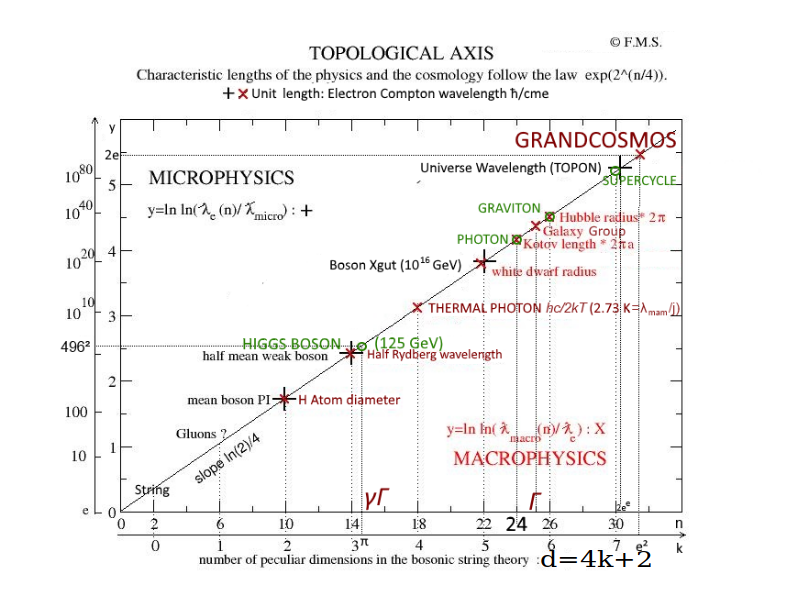
\includegraphics[width=0.5\textwidth]{./figures/figure}
\caption{Resonance-spectrum F(ν) computed for 15 motions of the largest, fast-spinning bodies of
the solar system. On horizontal axis is logarithm of frequency ν (in μHz), the dashed horizontal line
shows a 3σ C.L., and the primary peak corresponds to the best-commensurable period 9594(65) s.}
\label{fig:figure_label}
\end{figure}

\begin{figure}
\centering
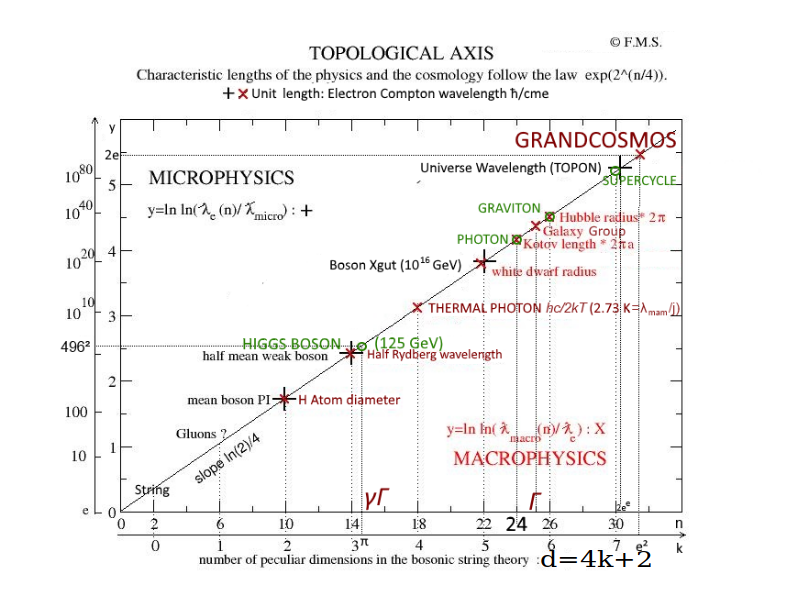
\includegraphics[width=0.5\textwidth]{./figures/figure}
\caption{Same as Fig. 2, for N = 11 sizes («diameters») of the solar system (with c = 1 and the π
factor for inner orbits). The highest peak corresponds to the spatial scale 9600(120) light sec.}
\label{fig:figure_label}
\end{figure}

\begin{figure}
\centering
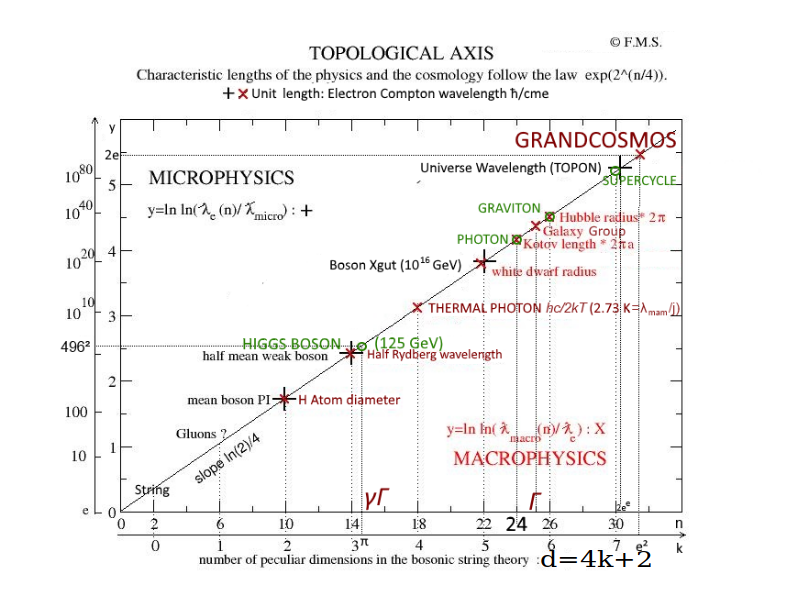
\includegraphics[width=0.5\textwidth]{./figures/figure}
\caption{Resonance-spectrum F 1 (ν), computed for N = 5746 binaries with periods < 5 days.
Horizontal axis gives logarithm of the trial frequency ν (in μHz), the dashed line indicates a 3σ
C.L., and the major peak corresponds to a timescale of 9590(70) s.}
\label{fig:figure_label}
\end{figure}

\begin{figure}
\centering
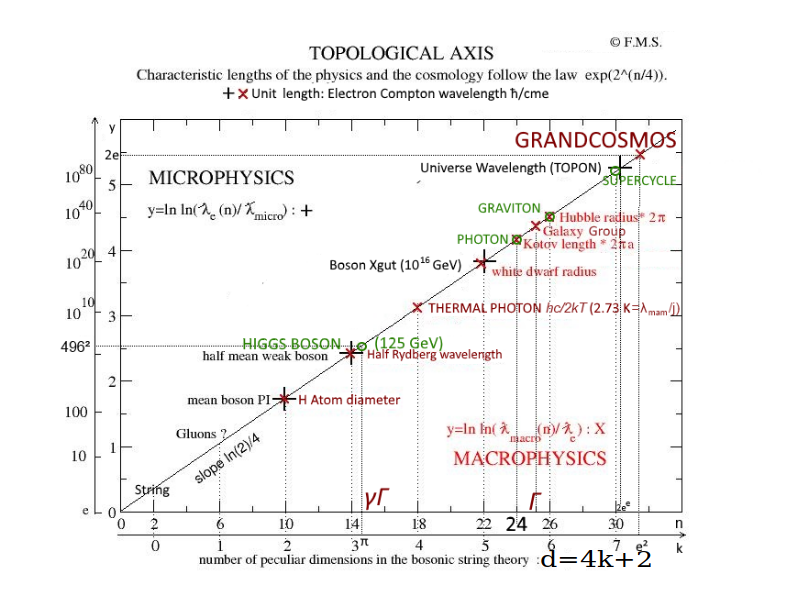
\includegraphics[width=0.5\textwidth]{./figures/figure}
\caption{Same as Fig. 4, for the F 2 (ν) spectrum, computed for N = 145 exoplanets with P < 1.5
days. The strongest peak of the composite commensurability corresponds to a period of 9640(115) s
at nearly 3.9σ significance (after Kotov, 2018).}
\label{fig:figure_label}
\end{figure}


\section {The Tifft, Arp and Pioneer effects}

Another unexplained effect is the 75(5) km/s periodicity in the galactic redshift [14]. Now this
speed v 1 is compatible with $c/v 1 ≈ √a w /a = F/a$, corresponding to the quantum resonance $$v n = nv 1 =n\hbar /r e m F $$, where $r e = \lambdabar e /a$ is the electron classical radius and $m F = m e √a w$ is the Fermi mass, close to the
mean DNA nucleotide mass [3].
The Halton Arp observations of chains of galaxies with different redshifts [15] was also
rejected. But it could be the sign of the galactic regeneration maintaining constant the visible
Universe mass: this is confirmed by the following confirmation of the invariance of the mean mass
density ρ c .
Much controversial is the Pioneer deceleration [16] $$g Pi ≈ 8.7 \cdot 10^{-10} ms^{-2}$$ . This corresponds to
the Pioneer time $$t Pi = c/g Pi ≈ 3.4 \cdot 10^{17} s$$, close to $$t = R/c ≈ 4.3587 \cdot 10^{17} s$$. The following section will show a connexion between the Kotov, Tifft and Pioneer effects.

\section {The Magical Logic of Prospective Dimensional Analysis}

Physical relations use principally physical quantities as monomials of type $Q = M^x L^y T^t$ , where
the three categories, M, L and T are Mass, Length and Time measurements, and where the exponents are
rational numbers. However, the addition of measures of different categories has no signification.
This seems at first sight illogical, since, fundamentally, a product is a sum of additions. So there
must be a hidden common nature for the 3 categories, mass, length and time. This sustains the
above single electron cosmic model [3]. Moreover, this mimics the Fundamental Principle of
Arithmetics, founded on prime numbers, but limited to the three M, L T categories. Indeed, with t =
R/c, summing the square of ln(M'/m e ), where M' = R'c 2 /2G is the critical mass in the above
holographic sphere representing the Grandcosmos, and the square of ln(R/\lambdabar e ) = ln(t/t e ), one gets, to
40 ppm:
$$ln 2 (M'/m e ) + ln 2 (R/\lambdabar e ) + ln 2 (t/t e ) ≈ ln 2 (R GC /\lambdabar e )$$
more precisely, to $10^{-8}$ , corresponding to $10{-7}$ precision on the above G value:
$$ln(√(ln 2 (M'/m e ) + ln 2 (R/\lambdabar e ) + ln 2 (t/t e ))) ≈ 2e – 1/2a$$
This is a dramatic geometrical confirmation for the visible Universe – Grandcosmos holographic
couple.
Another crucial point in Physics is the existence of invariant fundamental constants. Thus,
association of three of them must give characteristic values of M, L, T. So, approaching a domain in
Physics necessitates to calculate characteristic values (M, L, T), from the three universal constants
which are the most pertinent in the considered domain. This Prospective Dimensional Analysis is
largely used in Fluid Mechanics, were the equations are intractable, but is largely ignored in other
domains, because there is no real mathematical foundation, apart the above essential remarks. But
in virtue of the above Hierarchy Principle, the lack of theoretical justification is not a reason to
neglect Prospective Dimensional Analysis.
Now, the elimination of c in the above R formula means that the simplest basic dimensional
analysis starting from ħ, G and m, the Electron-Proton-Neutron mean mass gives a good
approximation for R/2. Indeed, in the Hypothesis of a Coherent Cosmos, it is logical to discard c
which is far two small a speed. This has not been observed during one century, since c is always
believed to be the single mandatory foundation of Space-Time. The warning of Poincaré, the true
discoverer of Relativity: 'use 4D space but do not confound Space and Time' has long been
forgotten, and physicist have unwisely put c = 1 in their equations.
In his three first minutes of cosmology, one of the author obtained the length:
$$l (ħ,G,m) = ħ 2 /Gm 3 ≈ R/2$$
but it took 9 years to get this published [12], and it appeared later [3] that m must be consideredmore precisely as the cubic root of the product m e m p m H . Moreover, the above critical condition
relies the time t = R/c and the mean mass density by the c-free formula $$ρ c = 3/8\pi Gt2 ≈ 9.41198 \cdot
10^{-27} kg m^{-3}$$ , So the mainstream idea of a temporal variability of the mean density ρ c cannot be to
sustain, meaning that ρ c must be considered as a fundamental constant. This writes:
$$t{\hbar,ρ c ,G} = 1/ρ c1/2 G 1/2 = (R/c) (8\pi/3) 1/2$$
This idea of ρ c being a fundamental constant permits to define R without any ambiguity: the
radius containing a critical mass. This means each point is the center of an equivalent black hole,
justifying the above application of the Bekenstein-Hawking entropy. Opponents would say that the
center of a black hole presents a singularity: that is indeed the case in the above flickering Space-
Mass-Time hypothesis. Other will argue that the flying galaxies cannot reach the celerity c at
horizon, but it must be reckognized that Relativity is a local theory, so do not apply in Cosmology.
Indeed, even General Relativity in unable to define what is a Galilean frame, while the Foucault
pendulus shows it directly, realizing the Cosmic Microwave Background frame, identified with the
Grandcosmos frame, as seen above.
Introducing the Fermi constant G F , the associated c-free length is very particular, to 1.7 %:
l{\hbar,ρ c ,G F } = \hbar/ρ c1/2 G F 1/2 ≈ 9.07154 10 9 m ≈ \lambdabar e 2/l P
Now, the following mandatory c-free times are close each over to 0.7 %:
$$T{\hbar,ρ c ,G F } = \hbar 4 /ρ c3/2 G F 5/2 ≈ 5.4829 10^{57} s$$
$$T'{\hbar,G,m} = \hbar 3 /G 2 m 5 ≈ 5.5224 \cdot 10^{57} s$$
This would be the periodic time of a Cycling Cosmos, which corresponds in the Topological Axis to
the holic dimension (see below) n = 30, to 4{percent}. Comparing T with the Kotov Non-Doppler Cosmic
Oscillation period t K ≈ 9600.60(2) s, one observes, to 0.04 {percent}:
$$T/t K ≈ O_M /√2$$
where O_M is the cardinal order of the Monster Group, the largest of the 26 sporadic groups, which is
suspected by some researchers to play a central role in Physics: indeed string theory allows a bridge
between apparently no-connected mathematical theories [17]. The simplest interpretation of T is the
cosmic period of all events, in a perfectly deterministic and periodic Cosmos.
Now, introducing the above Pioneer abnormal deceleration g PN , one gets the time: $t{G, m e , g PN }
= (Gm e /g PN 3 ) 1/4 = (t PN 3 t' e ) 1/4$ , where $t PN = c/g PN$ and $t' e = Gm e /c^3$ . This time is compatible with:
$t{G, m e , g PN } = t K /(F/a) 2$
where the above Tifft factor F/a appears. The implication of the time $t' e = Gm e /c^3 = 2.2568 × 10^{-66} s$
confirms the above Planck wall breakdown.

For updating nomenclature run the following commands:

makeindex Thesis-main.nlo -s nomencl.ist -o Thesis-main.nls

makeindex LettersClassification.nlo -s nomencl.ist -o LettersClassification.
